%\documentclass[a4paper, 12pt]{mwrep}
\documentclass[12pt,a4paper]{article}
\usepackage[polish]{babel}
\usepackage[T1]{fontenc}
\usepackage[utf8x]{inputenc}
\usepackage{hyperref}
\usepackage{url}
\usepackage[]{algorithm2e}
\usepackage{listings}
\usepackage{graphicx}
\usepackage{amsmath}
\graphicspath{
    {media/}
}

\usepackage{color}
\usepackage{listings}

\lstloadlanguages{% Check Dokumentation for further languages ...
	C,
	C++,
	csh,
	Java
}

\definecolor{red}{rgb}{0.6,0,0} % for strings
\definecolor{blue}{rgb}{0,0,0.6}
\definecolor{green}{rgb}{0,0.8,0}
\definecolor{cyan}{rgb}{0.0,0.6,0.6}

\lstset{
	language=csh,
	basicstyle=\footnotesize\ttfamily,
	numbers=left,
	numberstyle=\tiny,
	numbersep=5pt,
	tabsize=2,
	extendedchars=true,
	breaklines=true,
	frame=b,
	stringstyle=\color{blue}\ttfamily,
	showspaces=false,
	showtabs=false,
	xleftmargin=17pt,
	framexleftmargin=17pt,
	framexrightmargin=5pt,
	framexbottommargin=4pt,
	commentstyle=\color{green},
	morecomment=[l]{//}, %use comment-line-style!
	morecomment=[s]{/*}{*/}, %for multiline comments
	showstringspaces=false,
	morekeywords={ abstract, event, new, struct,
		as, explicit, null, switch,
		base, extern, object, this,
		bool, false, operator, throw,
		break, finally, out, true,
		byte, fixed, override, try,
		case, float, params, typeof,
		catch, for, private, uint,
		char, foreach, protected, ulong,
		checked, goto, public, unchecked,
		class, if, readonly, unsafe,
		const, implicit, ref, ushort,
		continue, in, return, using,
		decimal, int, sbyte, virtual,
		default, interface, sealed, volatile,
		delegate, internal, short, void,
		do, is, sizeof, while,
		double, lock, stackalloc,
		else, long, static,
		enum, namespace, string},
	keywordstyle=\color{cyan},
	identifierstyle=\color{red},
}
\usepackage{caption}
\DeclareCaptionFont{white}{\color{white}}
\DeclareCaptionFormat{listing}{\colorbox{blue}{\parbox{\textwidth}{\hspace{15pt}#1#2#3}}}
\captionsetup[lstlisting]{format=listing,labelfont=white,textfont=white, singlelinecheck=false, margin=0pt, font={bf,footnotesize}}


\addtolength{\hoffset}{-1.5cm}
\addtolength{\marginparwidth}{-1.5cm}
\addtolength{\textwidth}{3cm}
\addtolength{\voffset}{-1cm}
\addtolength{\textheight}{2.5cm}
\setlength{\topmargin}{0cm}
\setlength{\headheight}{0cm}

\begin{document}
	
	\title{Modelowanie i analiza systemów informatycznych\\
			\bigskip
			\large{dokumentacja projektu:} \\
			\large{System wspomagania decyzji}
		}
	\author{inż. Bartosz Ociepka
		\and inż. Beniamin Stecuła}
	\date{\today}
	
	\maketitle







	\newpage
\section*{Podział pracy}
Podział pracy był płynny, lecz z większym naciskiem na:
\begin{itemize}
	\item inż. Bartosz Ociepka -- backend, praktyka,
	\item inż. Beniamin Stecuła -- frontend, teoria, dokumentacja.
\end{itemize}
	
	
	
\section*{Udokumentowanie pracy}
	Dokumentowanie pracy odbyło się na kilka sposobów:
	\begin{itemize}
		\item utworzenie niniejszej dokumentacji,
		\item zarządzanie podziałem i wykonaniem zadań w serwisie Trello,
		\item przechowywanie kopii poprzednich wersji programu.
	\end{itemize}
	
	W ramach repozytorium każdy z nas wrzucał commity do swoim zadań \\
	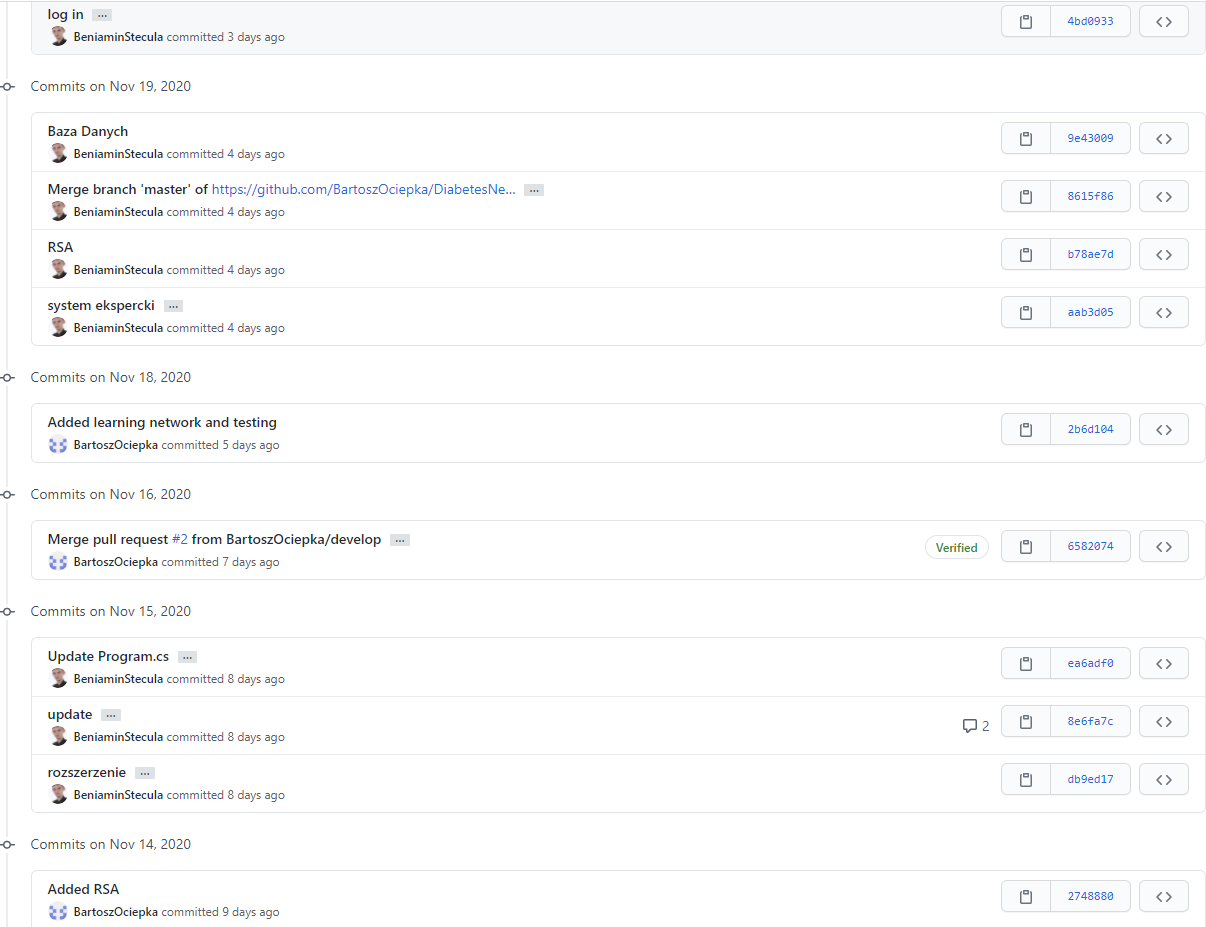
\includegraphics[width=0.9\linewidth]{media/githubProof}\\
	Całe repozytorium jest dostępne pod adresem \\https://github.com/BartoszOciepka/DiabetesNeuralNetwork
	
	
\section*{Instrukcja obsługi}
Niezalogowany użytkownik na start widzi menu, z którego może się zalogować, zarejestrować, sprawdzić próbkę lub wyjść.\\
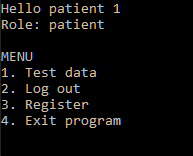
\includegraphics[width=0.5\linewidth]{media/menuPatient}\\
Po zalogowaniu jako doktor do menu dochodzi opcja dodania próbki, trenowania zbioru lub uruchomienia programu testującego, który sprawdza i pokazuje wyniki uczenia dla różnych konfiguracji sieci.\\
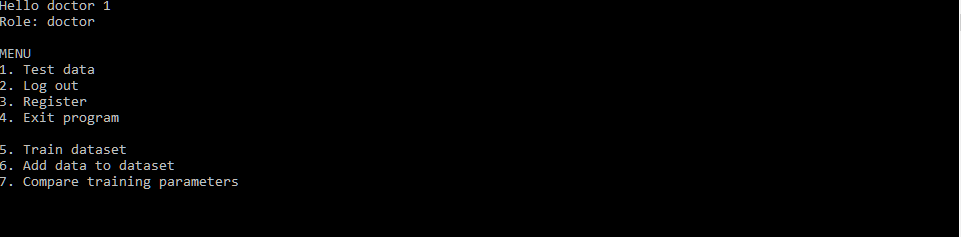
\includegraphics[width=0.9\linewidth]{media/menuDoctor}\\
Wchodząc w każdą opcję użytkownik jest prowadzony za rękę przez cały proces. W razie błędu lub podania niepoprawnych danych wyświetlany jest komunikat błędu.
	
\section*{Instrukcja wdrożenia}

	Aby wdrożyć projekt należy wykonać poniższą listę kroków:
	
	\begin{enumerate}
		\item zaimportowanie projektu w Visual Studio 2015,
		\item import danych do bazy danych MySql (dołączono plik dump.sql zawierający potrzebne tabele),
		\item zmiana connectionString w kodzie na odpowiadające używanej bazie,
		danych (dokonanie zmiany klas gdy używana jest inna baza niż MySql),
		\item uruchomienie projektu.
	\end{enumerate}
		
\section*{Baza danych}
Łączenie z bazą danych ma na stałe ustawione własności, które mogą być w razie potrzeby edytowane w klasie \emph{LinqToDbSettings.cs} we fragmencie:
	\begin{lstlisting}
	new ConnectionStringSettings
	{
		Name = "DiabetesDatabase",
		ProviderName = "MySql",
		ConnectionString = @"Server=localhost;Database=diabetes;Uid=;Pwd=;"
	};
	\end{lstlisting}


Diagram UML bazy danych został przedstawiony na rysunku \ref{fig:dbdiagram}.


\begin{figure}[h]
	\centering
	\centerline{
	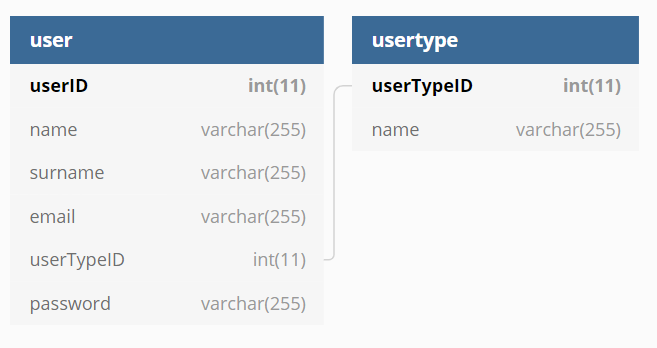
\includegraphics[width=0.9\linewidth]{media/dbdiagram}
	}
	\caption{Diagram klas.}
	\label{fig:dbdiagram}
\end{figure}



\section*{Komponenty systemu}
W naszym programie komponenty systemu uporządkowane są w odpowienich folderach o nazwach pokazujących jakie pliki tam znajdziemy. I tak mamy:\\
\begin{itemize}
\item Core - z głównymi elementami systemu, w naszym wypadku sieć neuronową\\
\item Authorization - pliki do logowania/rejestracji oraz trzymania ich stanu\\
\item Controllers - tutaj są kontrolery używane jako most między bazą danych a modelami\\
\item Helpers - klasy pomocnicze do walidacji i szyfrowania\\
\item Models - modele używane w programie\\
\item ORM - konfiguracja ORMa, którego używamy do komunikacji z bazą\\
\end{itemize}

Użyliśmy wzorca projektowego Singleton, dzięki temu nie musimy tworzyć obiektu gdy chcemy zwalidować dane lub je zaszyfrować. Można też uznać, że w ramach używania biblioteki AForge do sieci neuronowej używamy wzorca Fasada.\\\\

Nasza sieć neuronowa jest utworzona przy wykorzystaniu biblioteki AForge \\(http://www.aforgenet.com/framework/docs/). Nie jest to zbyt znana biblioteka, ale do jej wykorzystania przekonała nas bardzo dokładna dokumentacja.\\
Biblioteka udostępnia nam obiekt ActivationNetwork, który w konstruktorze bierze funkcję aktywacyjną, ilość wejsć sieci oraz tablicę neuronów w poszczególnych warstwach. W naszym wypadku za funkcję aktywacyjną wzieliśmy funkcję sigmoidalną z alfą równą 1.8 (taką wartość uznaliśmy za najlepszą w ramach testowania). Funkcja ta ma postać:
\begin{equation}
f(x)=\dfrac{1}{1+E^{-\alpha *x}}
\end{equation}
 Gdy już mamy utworzony obiekt sieci musimy ją nauczyc. Służy do tego klasa BackPropagationLearning (jak i inne, ale my będziemy uczyć sieć używając propagacji wstecznej).
	
\section*{Algorytm szyfrowania}
	
	
	W naszym programie do rejestracji i logowania użyliśmy stworzonej przez siebie klasy \emph{AuthorizationManager}, która zawiera metody \emph{LogIn(), Register(), LogOut()}.
	Szyfrowanie zaimplementowane zostało w klasie \emph{RSAHelper}, w której znajduje się cała logika szyfrowania opierająca się na klasie \emph{RSACryptoServiceProvider}.
	Do szyfrowania użyty został algorytm RSA (definicja oraz dwa wywołania):
	\begin{lstlisting}
		using (var rsa = new RSACryptoServiceProvider(2048))
		...
		User user = UserController.FindUserByEmailAndPassword(email, RSAHelper.encrypt(password));
		...
		User user = new User(name, surname, email, RSAHelper.encrypt(password), userTypeID);
	\end{lstlisting}

	



	Algorytm Rivesta-Shamira-Adlemana (RSA) to jeden z pierwszych i najpopularniejszych asymetrycznych algorytmów kryptograficznych o kluczu publicznym. Może być stosowany i do szyfrowania, i cyfrowego podpisywania plików.
	
	\smallskip
	Polega on na liczeniu funkcji Eulera dla dużych liczb pierwszych, a jego bezpieczeństwo opiera się na trudności faktoryzacji dużych liczb złożonych.
	
	\smallskip
	Każdy z rozmówców posiada parę kluczy: prywatny i publiczny. Pierwszy z nich służy do deszyfrowania wiadomości przychodzącej, a drugi do szyfrowania wychodzącej. Aby nawiązać komunikację rozmówcy muszą wymienić się swoimi kluczami publicznymi. Klucze prywatne nigdy nie są ujawniane.
	
	
	
	
	\subsection*{Generowanie kluczy}
	Generowanie pary kluczy:
	\begin{itemize}
		\item losujemy duże liczby pierwsze $p$ i $q$ odległe, lecz o zbliżonej długości,
		\item $n = pq$,
		\item obliczamy funkcję Eulera dla $n$: $ \varphi (n)=(p-1)(q-1) $,
		\item wybieramy liczbę $e$, gdzie:  $(1 < e < \varphi(n))$, która jest względnie pierwsza z $\varphi(n)$,
		\item $d ≡ e−1 (mod \varphi(n))$, czyli: $d⋅e ≡ 1 (mod \varphi(n))$,
		\item kluczem publicznym jest para liczb $(n, e)$, a prywatnym $(n, d)$.
	\end{itemize}
	
	
	\subsection*{Szyfrowanie i deszyfrowanie}
	Korzystamy z dwóch wzorów:
	\begin{itemize}
		\item wiadomość dzielimy na bloki $m$ o wartości nie większej niż $n$, a następnie: $c\equiv m^{e}{\pmod {n}}$,
		\item zaszyfrowane bloki $c$ deszyfrujemy wzorem: $m\equiv c^{d}{\pmod {n}}$.
	\end{itemize}
	
	
	
	
	
	
	
	
	
	
\section*{System ekspercki}

	W dziale sztucznej inteligencji systemem eksperckim (Expert System -- ES) nazywa się system komputerowy, który emuluje podejmowanie decyzji przez ludzkiego specjalistę z danej dziedziny. Odzwierciedla procesy myślowe na zasadzie działania ludzkiego mózgu.
	
	Do rozwiązań wykorzystujących ES zaliczamy:
	\begin{itemize}
		\item systemy agentowe,
		\item agenty programowe,
		\item eksplorację danych,
		\item wspomaganie twórczego myślenia,
		\item ontologie systematyzujące wiedzę.
	\end{itemize}
	\bigskip
	
	ES powinien zawierać trzy charakterystyczne, podstawowe cechy:
	\begin{itemize}
		\item bazy wiedzy -- schematycznie zapisane informacje uzyskane od ludzkich ekspertów w danej dziedzinie,
		\item procedury wnioskujące -- odzwierciedlające wnioskowanie symboliczne, które jest charakterystyczne dla funkcjonowania ludzkiego mózgu,
		\item zdolność do poszerzania wiedzy -- umożliwienie ciągłego rozwoju systemu w przypadku stale napływających nowych informacji koniecznych do uwzględnienia aby otrzymywać stale aktualne wyniki zgodne z nowym stanem wiedzy w dziedzinie.
	\end{itemize}
	\bigskip
	
	Struktura ES składa się z sześciu podstawowych elementów:
	\begin{itemize}
		\item baza wiedzy -- składająca się ze zbioru reguł,
		\item baza danych -- zawierająca dane obiektów, wartości, przypadki i hipotezy,
		\item procedury wnioskowania -- jest to maszyna wnioskująca,
		\item procedury objaśniania -- tłumaczą strategię wnioskowania,
		\item procedury sterowania dialogiem -- funkcje wejścia/wyjścia sterujące programem i wyznaczające zadania, które ma wykonać
		\item procedury zarządzania wiedzą -- pozwalają na modyfikację oraz rozszerzanie, pozyskiwanie wiedzy.
	\end{itemize}
	
	
	
	%ES zazwyczaj działa na zasadzie rozpatrywania warunków if-else.
	
	Implementując kod programu i tworząc samemu kod ekspertowy doszliśmy do pewnych wniosków na temat zalet i wad systemów eksperckich:\\
	Zalety to na pewno szybkość przetwarzania danych. Człowiekowi zajęło by to nieporównywanie więcej czasu niż komputerowi. Do tego sieć potrafi zauważyć powiązanie, które człowiek pominie albo nie zauważy.\\
	Wady to przede wszystkim brak zdrowego rozsądku. Dla komputera liczby to liczby więc błędne dane czy dane na logikę wskazujące na pewne rozwiązanie nie zwrócą jego uwagi. Dochodzi do tego możliwość przeuczenia sieci, błędne dopasowanie parametrów sieci lub zbyt mały zbiór danych i mamy rozwiązanie, które jest bardzo potężne, ale wymaga uwagi i wiedzy aby poprawnie zaimplementować.
	
	
	
	
	
\section*{Sieć neuronowa}
	
	Siecią neuronową nazywa się struktury matematyczne z ich programowymi implementacjami. Realizują obliczenia i przetwarzają sygnały drobnymi elementami nazywanymi sztucznymi neuronami, które wykonują proste operacje na otrzymanych danych wejściowych.
	
	Zasada działania opiera się na mózgu składającym się z naturalnych neuronów, łączących je synaps oraz układów nerwowych. 
	
	Typy sieci neuronowych:
	\begin{itemize}
		\item jednokierunkowe -- bez sprzężenia zwrotnego,
		\item rekurencyjne -- ze sprzężeniem zwrotnym,
		\item samoorganizujące się mapy -- sieci Kohonena, gdzie neurony są stowarzyszone ze współrzędnymi na prostej lub przestrzeni wyższego rzędu.
	\end{itemize}


	\subsection*{Dobieranie parametrów w programie}
	
	W naszym programie do dobierania optymalnych parametrów służy metoda \emph{compareTrainingParameters()}. Iteruje ona, zgodnie z parametrami po kolejnej liczbie warstw oraz po liczbach neuronów w każdej warstwie. Istnieje jednak warunek, że w kolejnej warstwie nie może być więcej neuronów niż w poprzedniej.
	
	
	\begin{lstlisting}
		internal static void compareTrainingParameters()
		{
			//Random rand = new Random();
			maxNeurons = 16;
			minNeuronsBefore = maxNeurons;
			int maxLayers = 3;
			
			Console.WriteLine("Max neurons in a layer:\t" + maxNeurons);
			Console.WriteLine("Max number of layers:\t" + maxLayers);
			Console.WriteLine("Alpha:\t" + alpha);
			Console.WriteLine("Max error accepted:\t" + maxError);
			
			for (layersNumber = 2; layersNumber<=maxLayers; layersNumber++)
			{
				Console.WriteLine("\nCurrent number of layers:\t" + layersNumber);
				
				int[] neuronsTable = new int[layersNumber];
				neuronsTable[layersNumber - 1] = 1;
				
				// generate all possibilities for a set of layers
				//neurons[i] = rand.Next(1, maxNeurons);
				incrementNeuron(0, neuronsTable, minNeuronsBefore);
			}
		}
		private static void incrementNeuron(int layer, int[] neuronsTable, int minNeuronsBefore)
		{
			double error;
			// last layer with neurons
			if(layer==layersNumber-2)
			{
				for(int neu=1; neu<=minNeuronsBefore; neu++)
				{
					neuronsTable[layer] = neu;
					
					int timesEachValuesAreTested = 1;
					
					Console.Write("Testing: ");
					foreach (int n in neuronsTable) Console.Write(n + " ");
					
					error = trainNetwork(neuronsTable, alpha, false, timesEachValuesAreTested);
					if (error <= maxError)
					{
						Console.WriteLine("\tError: " + error);
					}
					else
					{
						Console.WriteLine("\tError too much");
					}
				}
				//foreach (int n in neuronsTable) Console.Write(n + " ");
				Console.WriteLine();
			}
			// increment and next number
			else
			{
				for (int neu = 1; neu <= minNeuronsBefore; neu++)
				{
					neuronsTable[layer] = neu;
					if (minNeuronsBefore > neu)
					incrementNeuron(layer+1, neuronsTable, neu);
					else
					incrementNeuron(layer + 1, neuronsTable, minNeuronsBefore);
				}
				//foreach (int n in neuronsTable) Console.Write(n + " ");
				//Console.WriteLine();
				return;
			}
		}
	\end{lstlisting}
	
	

\section*{Przykładowy kod z aplikacji z testami}

RSAHelper.cs
\begin{lstlisting}
using System;
using System.Security.Cryptography;
using System.Text;

namespace DiabetesNeuralNetwork
{
	public class RSAHelper
	{
		public static string containerName = "defaultContainerName";
		public static string encrypt(string message)
		{
			var bytesToEncrypt = Encoding.UTF8.GetBytes(message);

			using (var rsa = new RSACryptoServiceProvider(2048))
			{
				try
				{
					rsa.FromXmlString(RSAHelper.getPublicKeyFromContainer());
					var encryptedData = rsa.Encrypt(bytesToEncrypt, true);
					var base64Encrypted = Convert.ToBase64String(encryptedData);
					return base64Encrypted;
				}
				finally
				{
					rsa.PersistKeyInCsp = false;
				}
			}
		}

		public static string decrypt(string message)
		{
			var bytesToDescrypt = Encoding.UTF8.GetBytes(message);

			using (var rsa = new RSACryptoServiceProvider(2048))
			{
				try
				{
					rsa.FromXmlString(RSAHelper.getPrivateKeyFromContainer());

					var resultBytes = Convert.FromBase64String(message);
					var decryptedBytes = rsa.Decrypt(resultBytes, true);
					var decryptedData = Encoding.UTF8.GetString(decryptedBytes);
					return decryptedData.ToString();
				}
				finally
				{
					rsa.PersistKeyInCsp = false;
				}
			}
		}

		// Run this method before any encryption.
		// This method adds a new key container and saves it on the machine. That way the public and private keys are the same each run.
		public static void addKeysToContainer()
		{
			var parameters = new CspParameters
			{
				KeyContainerName = RSAHelper.containerName
			};

			var rsa = new RSACryptoServiceProvider(parameters);

			Console.WriteLine("Added new key provider to default container");
		}

		public static string getPublicKeyFromContainer()
		{
			var parameters = new CspParameters
			{
				KeyContainerName = containerName
			};
			
			var rsa = new RSACryptoServiceProvider(parameters);
			var publicKey = rsa.ExportParameters(false); //Generowanie klucza publiczny
			string publicKeyString = RSAHelper.GetKeyString(publicKey);

			// Display the key information to the console.
			Console.WriteLine($"Public key retrieved from container");

			return publicKeyString;
		}

		public static string getPrivateKeyFromContainer()
		{
			var parameters = new CspParameters
			{
				KeyContainerName = containerName
			};

			var rsa = new RSACryptoServiceProvider(parameters);
			var privateKey = rsa.ExportParameters(true); //Generowanie klucza publiczny
			string privateKeyString = RSAHelper.GetKeyString(privateKey);

			Console.WriteLine("Private key retrieved from container");

			return privateKeyString;
		}
		public static string GetKeyString(RSAParameters key)
		{
			var stringWriter = new System.IO.StringWriter();
			var xmlSerializer = new System.Xml.Serialization.XmlSerializer(typeof(RSAParameters));
			xmlSerializer.Serialize(stringWriter, key);
			return stringWriter.ToString();
		}
	}
}

\end{lstlisting}

UserType.cs
\begin{lstlisting}
using System.Collections.Generic;
using LinqToDB.Mapping;

namespace DiabetesNeuralNetwork.Models
{
	[Table(Name = "UserType")]
	public class UserType
	{
		[PrimaryKey, Identity]
		public int userTypeID;
		[Column(Name = "name"), NotNull]
		public string name { get; set; } 
		List<User> users { get; set; }

		public override string ToString()
		{
			return this.userTypeID + " " + this.name;
		}
	}
}

\end{lstlisting}

User.cs
\begin{lstlisting}
using LinqToDB.Mapping;

namespace DiabetesNeuralNetwork
{
	[Table(Name = "User")]
	public class User
	{
		[PrimaryKey, Identity]
		public int userID;
		[Column(Name = "name"), NotNull]
		public string name;
		[Column(Name = "surname"), NotNull]
		public string surname;
		[Column(Name = "email"), NotNull]
		public string email;
		[Column(Name = "userTypeID"), NotNull]
		public int userTypeID;
		[Column(Name = "password"), NotNull]
		public string password;

		public User()
		{

		}
		public User(string name, string surname, string email, string password, int userTypeID)
		{
			this.name = name;
			this.surname = surname;
			this.email = email;
			this.password = password;
			this.userTypeID = userTypeID;
		}

		public override string ToString()
		{
			return this.name + " " + this.surname + " " + this.email;
		}
	}
}

\end{lstlisting}

AuthorizationManager.cs
\begin{lstlisting}
using DiabetesNeuralNetwork.Controllers;
using System;

namespace DiabetesNeuralNetwork
{
	class AuthorizationManager
	{
		public static void LogIn()
		{
			Console.WriteLine("Email:");
			string email = Console.ReadLine();
			Console.WriteLine("Password:");

			var password = readPassword();

			User user = UserController.FindUserByEmailAndPassword(email, RSAHelper.encrypt(password));
			if(user == null) {
				Console.WriteLine("Incorrect credentials");
			}
			else
			{
				LogInUser(user);
				Console.WriteLine("Hi " + user.name + "! You were successfully logged in.");
			}
		}

		public static void LogInUser(User user)
		{
			LoginStatus.IsLoggedIn = true;
			LoginStatus.LoggedInUser = user;
		}

		public static void Register()
		{
			try
			{
				Console.WriteLine("What user type to register:");
				UserTypeController.GetAll().ForEach(i => Console.WriteLine("{0}\t", i));
				int userTypeID = Int32.Parse(Console.ReadLine());
				Console.WriteLine("Name:");
				string name = Console.ReadLine();
				Console.WriteLine("Surname:");
				string surname = Console.ReadLine();
				Console.WriteLine("Email:");
				string email = Console.ReadLine();
				Console.WriteLine("Password:");
				string password = readPassword();


				Validator.ValidateUser(name, surname, email, password, userTypeID);
				User user = new User(name, surname, email, RSAHelper.encrypt(password), userTypeID);
				UserController.Insert(user);
				LogInUser(user);
				Console.WriteLine("Successfully registered new user");
			}
			catch (Exception ex)
			{
				Console.WriteLine(ex.Message);
			}
		}

        private static string readPassword()
        {
			var password = string.Empty;
			ConsoleKey key;
			do
			{
				var keyInfo = Console.ReadKey(intercept: true);
				key = keyInfo.Key;

				if (key == ConsoleKey.Backspace && password.Length > 0)
				{
					Console.Write("\b \b");
					password = password.Remove(password.Length - 1);
				}
				else if (!char.IsControl(keyInfo.KeyChar))
				{
					Console.Write("*");
					password += keyInfo.KeyChar;
				}
			} while (key != ConsoleKey.Enter);
			Console.WriteLine();
			
			return password;
		}

        public static void LogOut()
		{
			LoginStatus.IsLoggedIn = false;
			LoginStatus.LoggedInUser = null;
			Console.WriteLine("Successfully logged out");
		}



	}
}
\end{lstlisting}

Przykładowe testy:
\begin{lstlisting}
		[TestMethod]
		public void TestRSACorrectlyEncryptsAndDecrypts()
		{
			string testString = "Ala ma kota";

			string encryptedText = RSAHelper.encrypt(testString);

			Assert.AreEqual(testString, RSAHelper.decrypt(encryptedText), false, "Original text and same text after encrypt and decrypt are not the same");
		}
		[TestMethod]
		public void TestRSAEncryptsTheSameEachTime()
		{
			string testString = "Ala ma kota";

			string encryptedText = RSAHelper.encrypt(testString);
			string anotherEncryptedText = RSAHelper.encrypt(testString);

			Assert.AreEqual(RSAHelper.decrypt(encryptedText), RSAHelper.decrypt(anotherEncryptedText), false, "Not the same results when encrypting and decrypting the same string");
		}
		[TestMethod]
		public void testUserValidationCorrect()
		{
			string name = "test";
			string surname = "test";
			string password = "test";

			Validator.ValidateName(name);
			Validator.ValidateSurname(surname);
			Validator.ValidatePassword(password);
		}

		[TestMethod]
		[ExpectedException(typeof(Exception), "Empty name should not pass validation")]
		public void testUserValidationIncorrect()
		{
			Validator.ValidateName("");
		}
\end{lstlisting}

\section*{Wyglad programu}

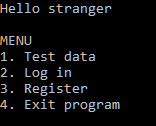
\includegraphics[width=0.4\linewidth]{media/program1}
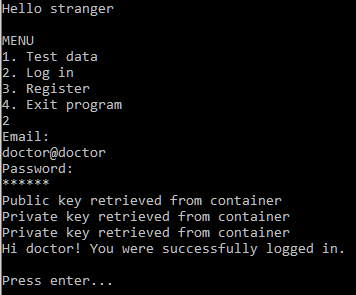
\includegraphics[width=0.4\linewidth]{media/program2}\\
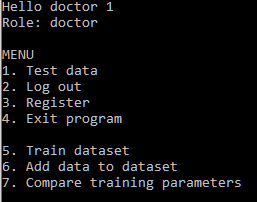
\includegraphics[width=0.4\linewidth]{media/program3}
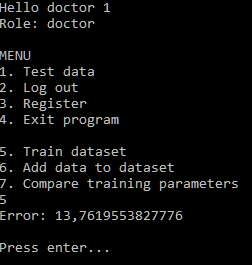
\includegraphics[width=0.4\linewidth]{media/program4}\\
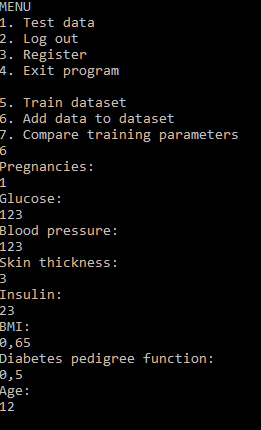
\includegraphics[width=0.4\linewidth]{media/program5}
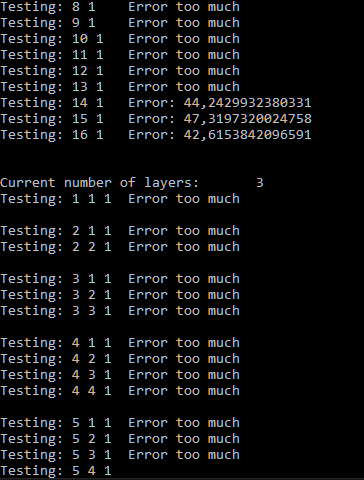
\includegraphics[width=0.4\linewidth]{media/program6}\\

\end{document}
